
\begin{frame}
\frametitle{Sectional Curvature}
\begin{block}{Definition of Sectional Curvature}
Let $M$ be a Riemann manifold. Let $\sigma$ be a two dimensional subspace of $T_pM$ Let $(v,w)$ be a basis of $\sigma$. Then the scalar curvature is defined as
\begin{align}
\label{def}
K(v,w)=\bfrac{\inner{R(v,w)w,v)}}{\abs{v\wedge w}^2}
\end{align}
\end{block}
\pause
Note that the above definition of the sectional curvature is independent of the choice of basis $(v,w)$ and is thus a property of the plane $\sigma$ alone. This will be proven in the slides to come.
\end{frame}

\begin{frame}
\frametitle{Intuitive Version of Sectional Curvature}
Here we will intuitively see why the sectional curvature takes the form as given in \ref{def}. Note that the intuitive version presented in these slides is a culmination of various sources on the internet presenting several viewpoints on the topic.
\pause
I will be using geodesics as the starting point for the intuition behind curvature. Note that the definition of geodesic is a curve on a surface along which the distance between two points is the shortest. This can also be interpreted as the path that parallel transport of a vector along itself takes.
\pause
We will use a vector field of the tangent vectors on the family of geodesics, denoted by $V$ and the vector field orthogonal to it, denoted by $S$. Note that we can use the vectors in $S$ to estimate the distance between geodesics at a given point.
\end{frame}

\begin{frame}
\frametitle{Figure for Intuitive Version of Sectional Curvature}
\begin{figure}[!htb]
	\centering
   \begin{minipage}{0.8\textwidth}
     \centering
     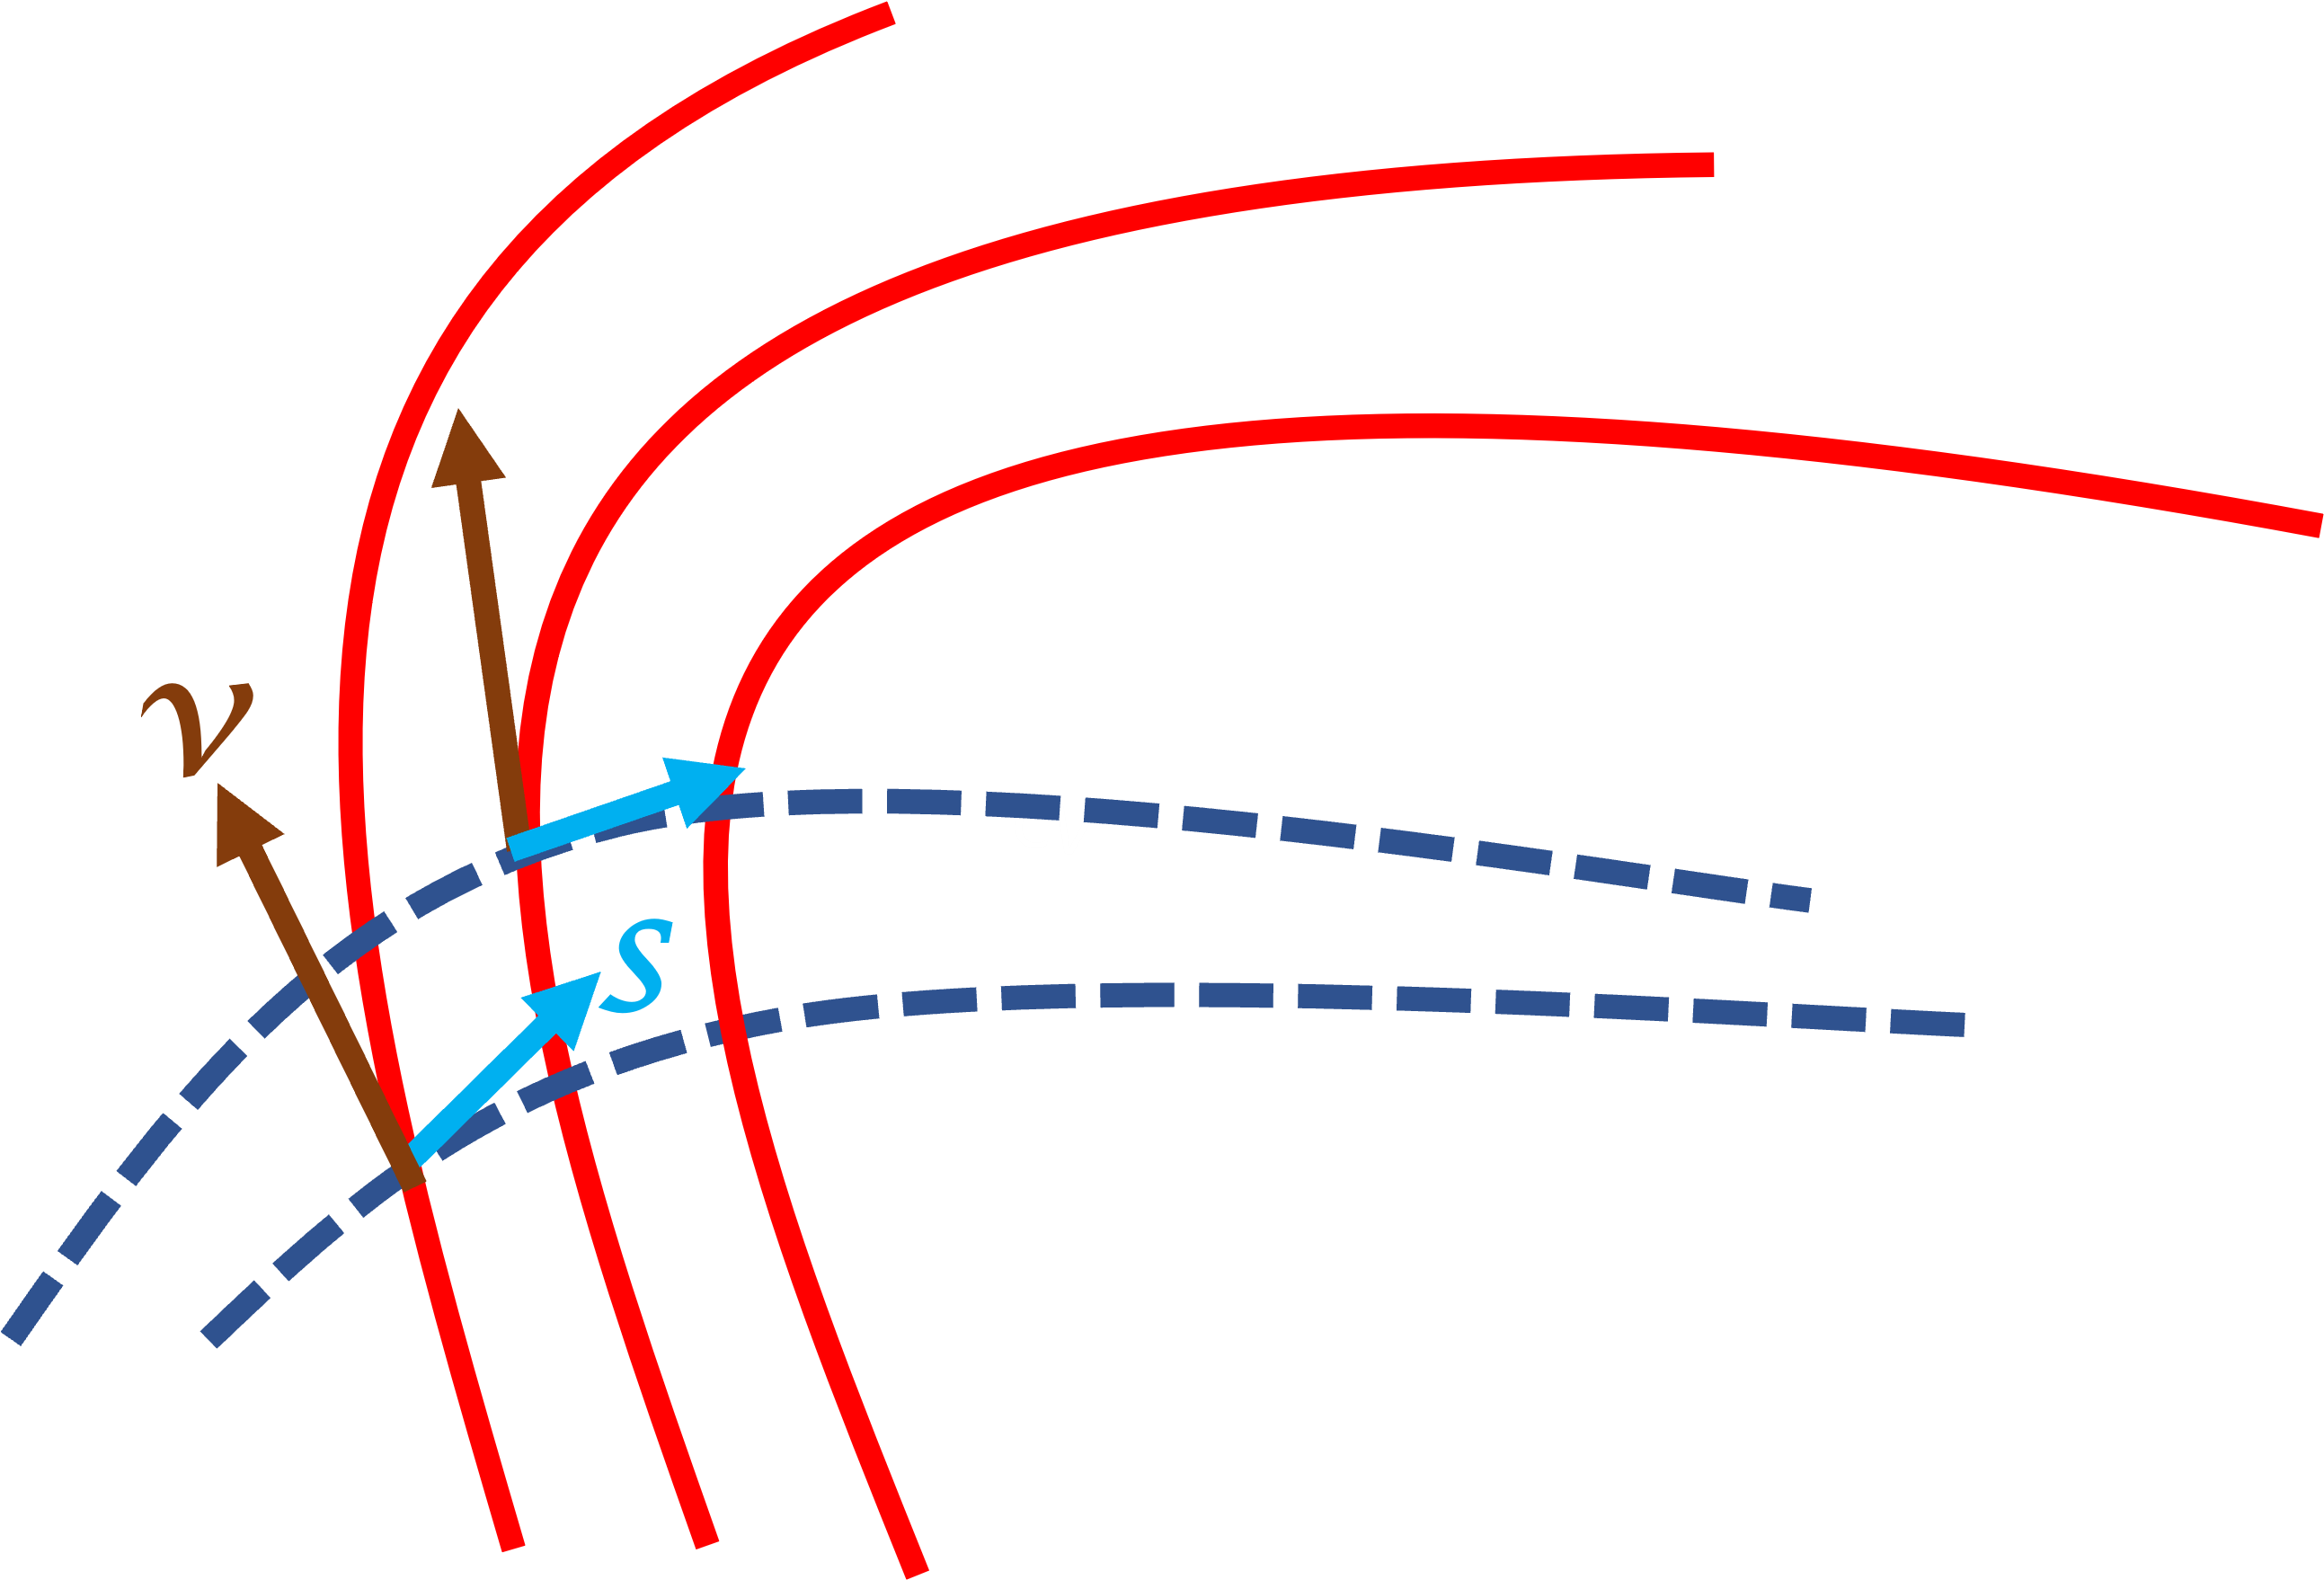
\includegraphics[width=0.8\linewidth]{img01.png}
     \caption{{Geodesics on some arbitrary surface. Note that $\mathbf{v}$ indicates the tangent vector to the geodesic $\mathbf{s}$ is the orthogonal vector that measures the distance between two geodesics.}}
     \label{fig:01}
   \end{minipage}
\end{figure}
\end{frame}
%
%
\begin{frame}
\frametitle{Getting into the Math behind Curvature}
We will start with some basic assumptions. Let $(M,g)$ be our Riemann Manifold.
\begin{itemize}
\item We choose $\nabla$ to be the connection whose torsion is $0$.
\item We will let the lie brackets of the vector fields $V$ and $S$.
\end{itemize}
\pause
Recall that in multi-variable calculus, we often used the second derivative to check curvature. This works because the second derivative measures the change of change of function. Change of function can occur even without curvature since the change can be uniform (linear). We will apply an analogous concept here by replacing the double derivative with double covariant derivative of the vector field $V$.
\pause
Note that the geodesic equation is given as the vector field whose parallel transport along itself is zero (i.e., covariant derivative with respect to itself is zero).
Thus, we have
\begin{align}
\nabla_{\vec{v}} \vec{v}=0
\end{align}
\end{frame}

\begin{frame}
\frametitle{Math behind Curvature}
Continuing,
\begin{align}
\nabla_{\vec{v}} \vec{v}=0
\end{align}
Taking covariant derivative with respect to $\vec{s}$ on both sides,
\begin{align}
\nabla_{\vec{s}}\nabla_{\vec{v}} \vec{v}&=0\\
\Rightarrow \nabla_{\vec{s}}\nabla_{\vec{v}} \vec{v}-\nabla_{\vec{v}}\nabla_{\vec{s}} \vec{v}+\nabla_{\vec{v}}\nabla_{\vec{s}} \vec{v}&=0
\end{align}
Using the definition of Riemann Curvature, the above equation reduces to
\begin{align}
\label{main_eq}
R(\vec{s},\vec{v})\vec{v}+\nabla_{\vec{v}}\nabla_{\vec{v}} \vec{s}=0
\end{align}
\end{frame}


\begin{frame}
\frametitle{More Figures}
\begin{figure}[!htb]
	\centering
   \begin{minipage}{0.3\textwidth}
     \centering
     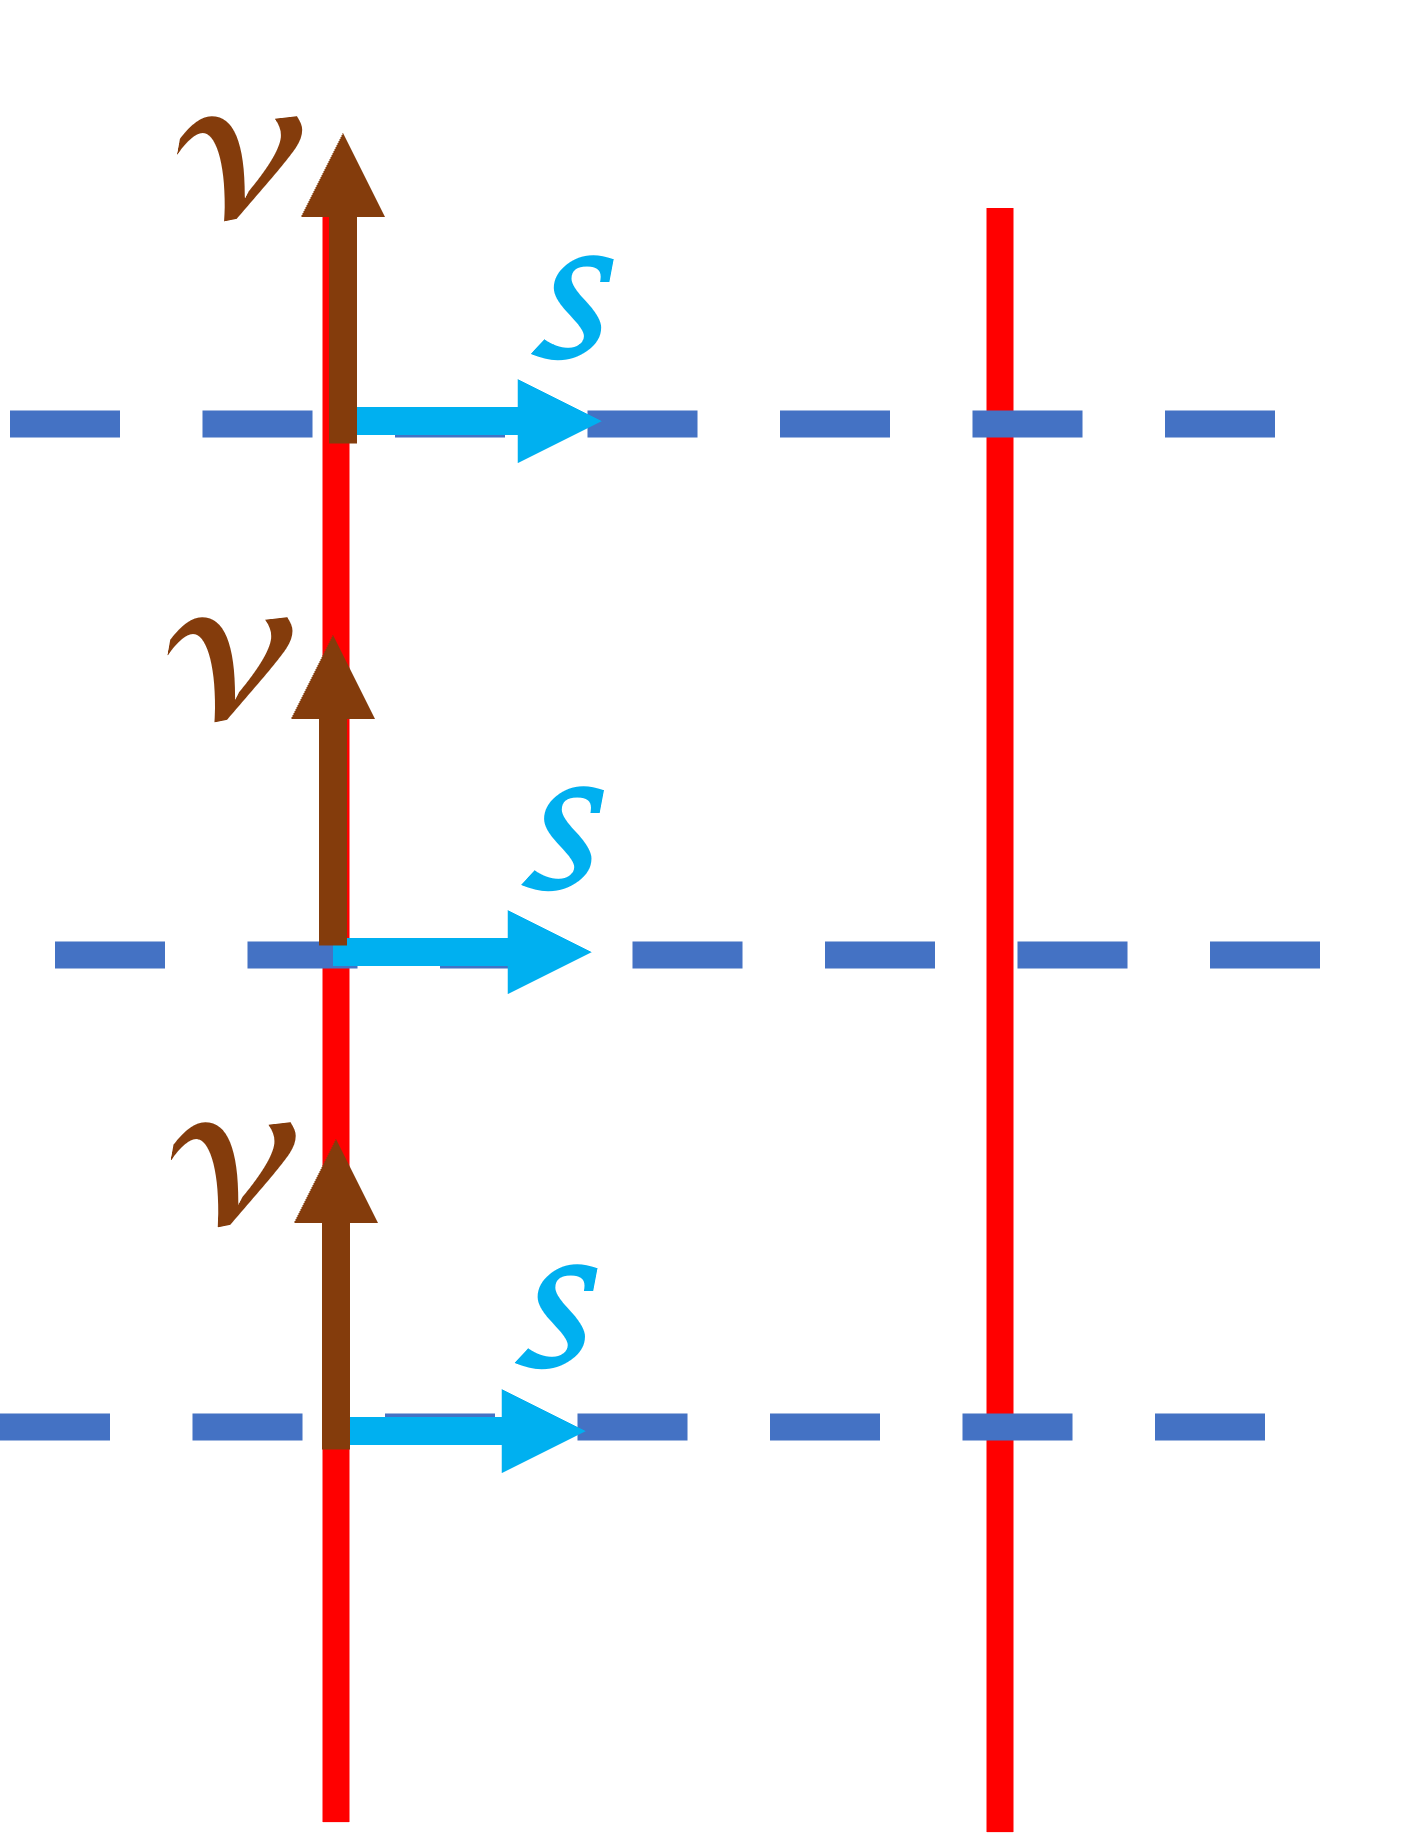
\includegraphics[width=\linewidth]{img02.png}
     \caption{{Case I: We have straight geodesics}}
     \label{fig:02}
   \end{minipage}
   \begin{minipage}{0.3\textwidth}
     \centering
     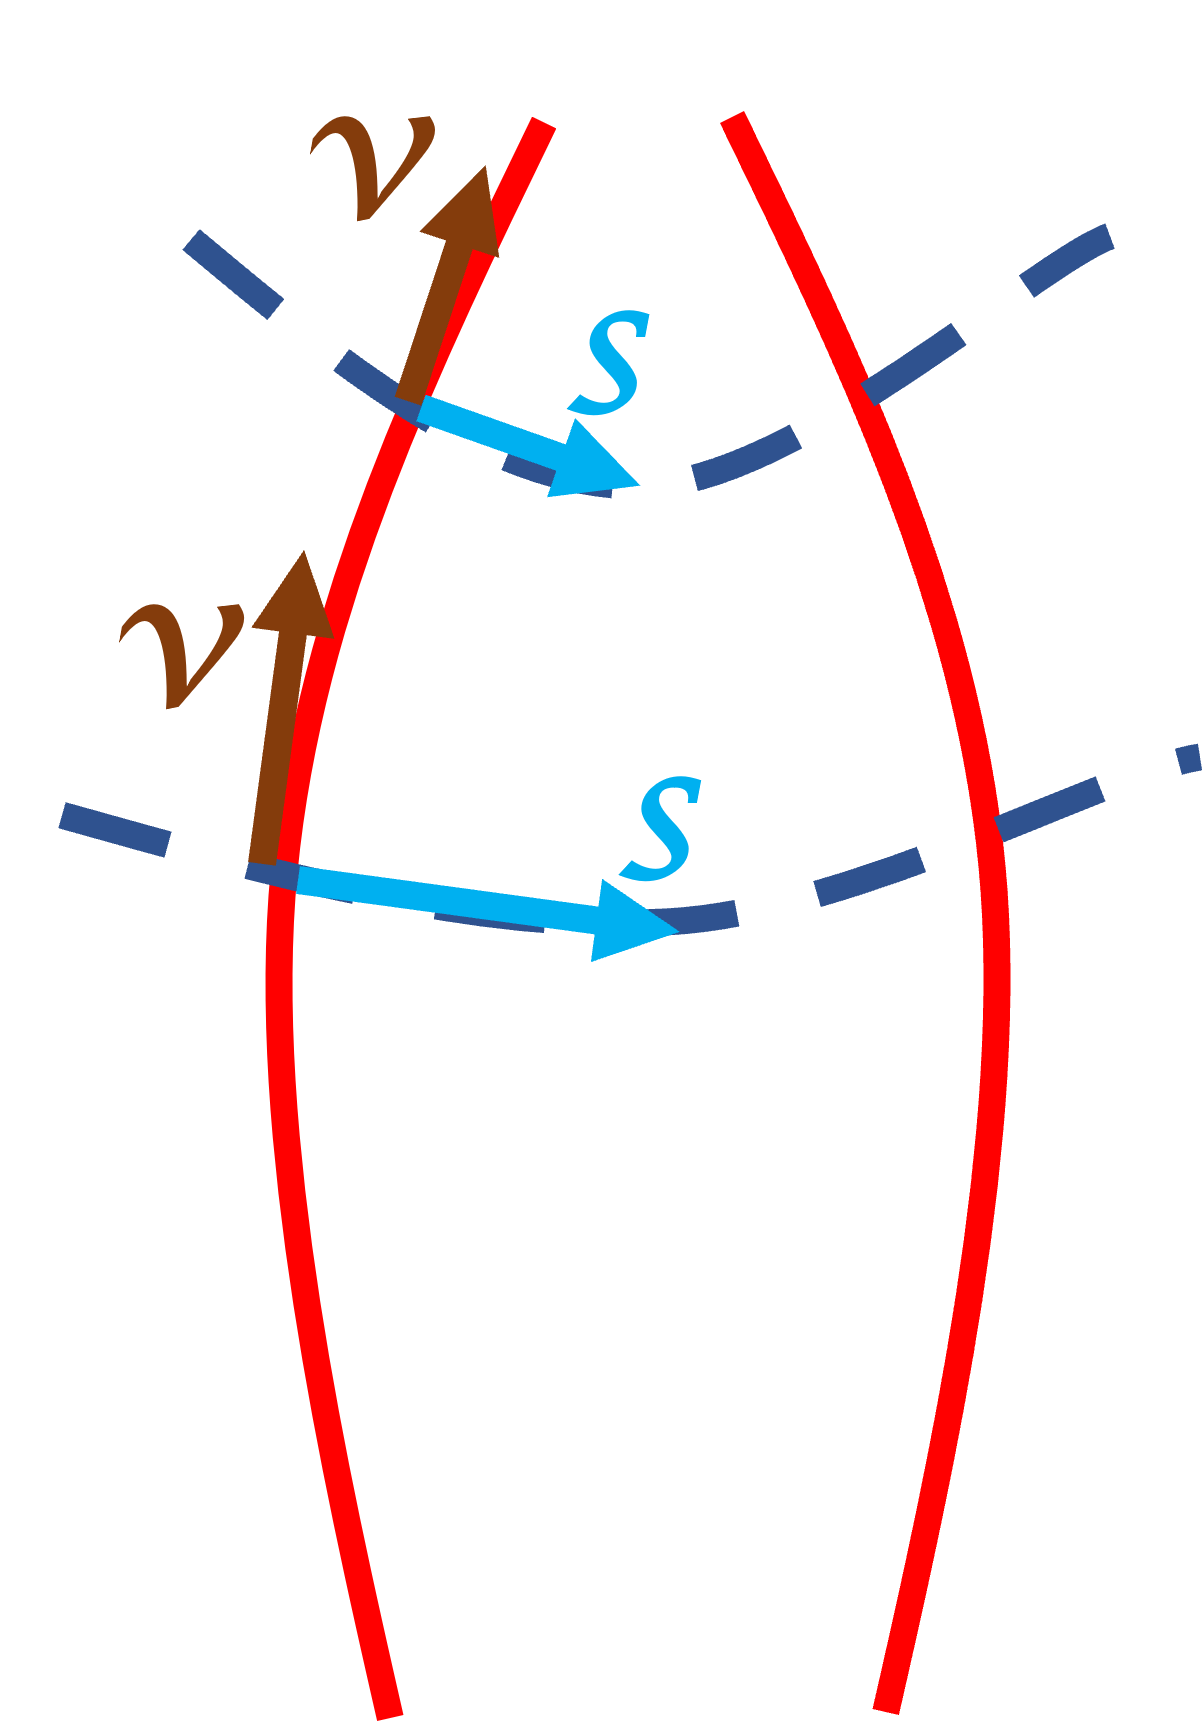
\includegraphics[width=\linewidth]{img03.png}
     \caption{{Case II: We have converging geodesics (positive curvature)}}
     \label{fig:03}
   \end{minipage}
   \begin{minipage}{0.3\textwidth}
     \centering
     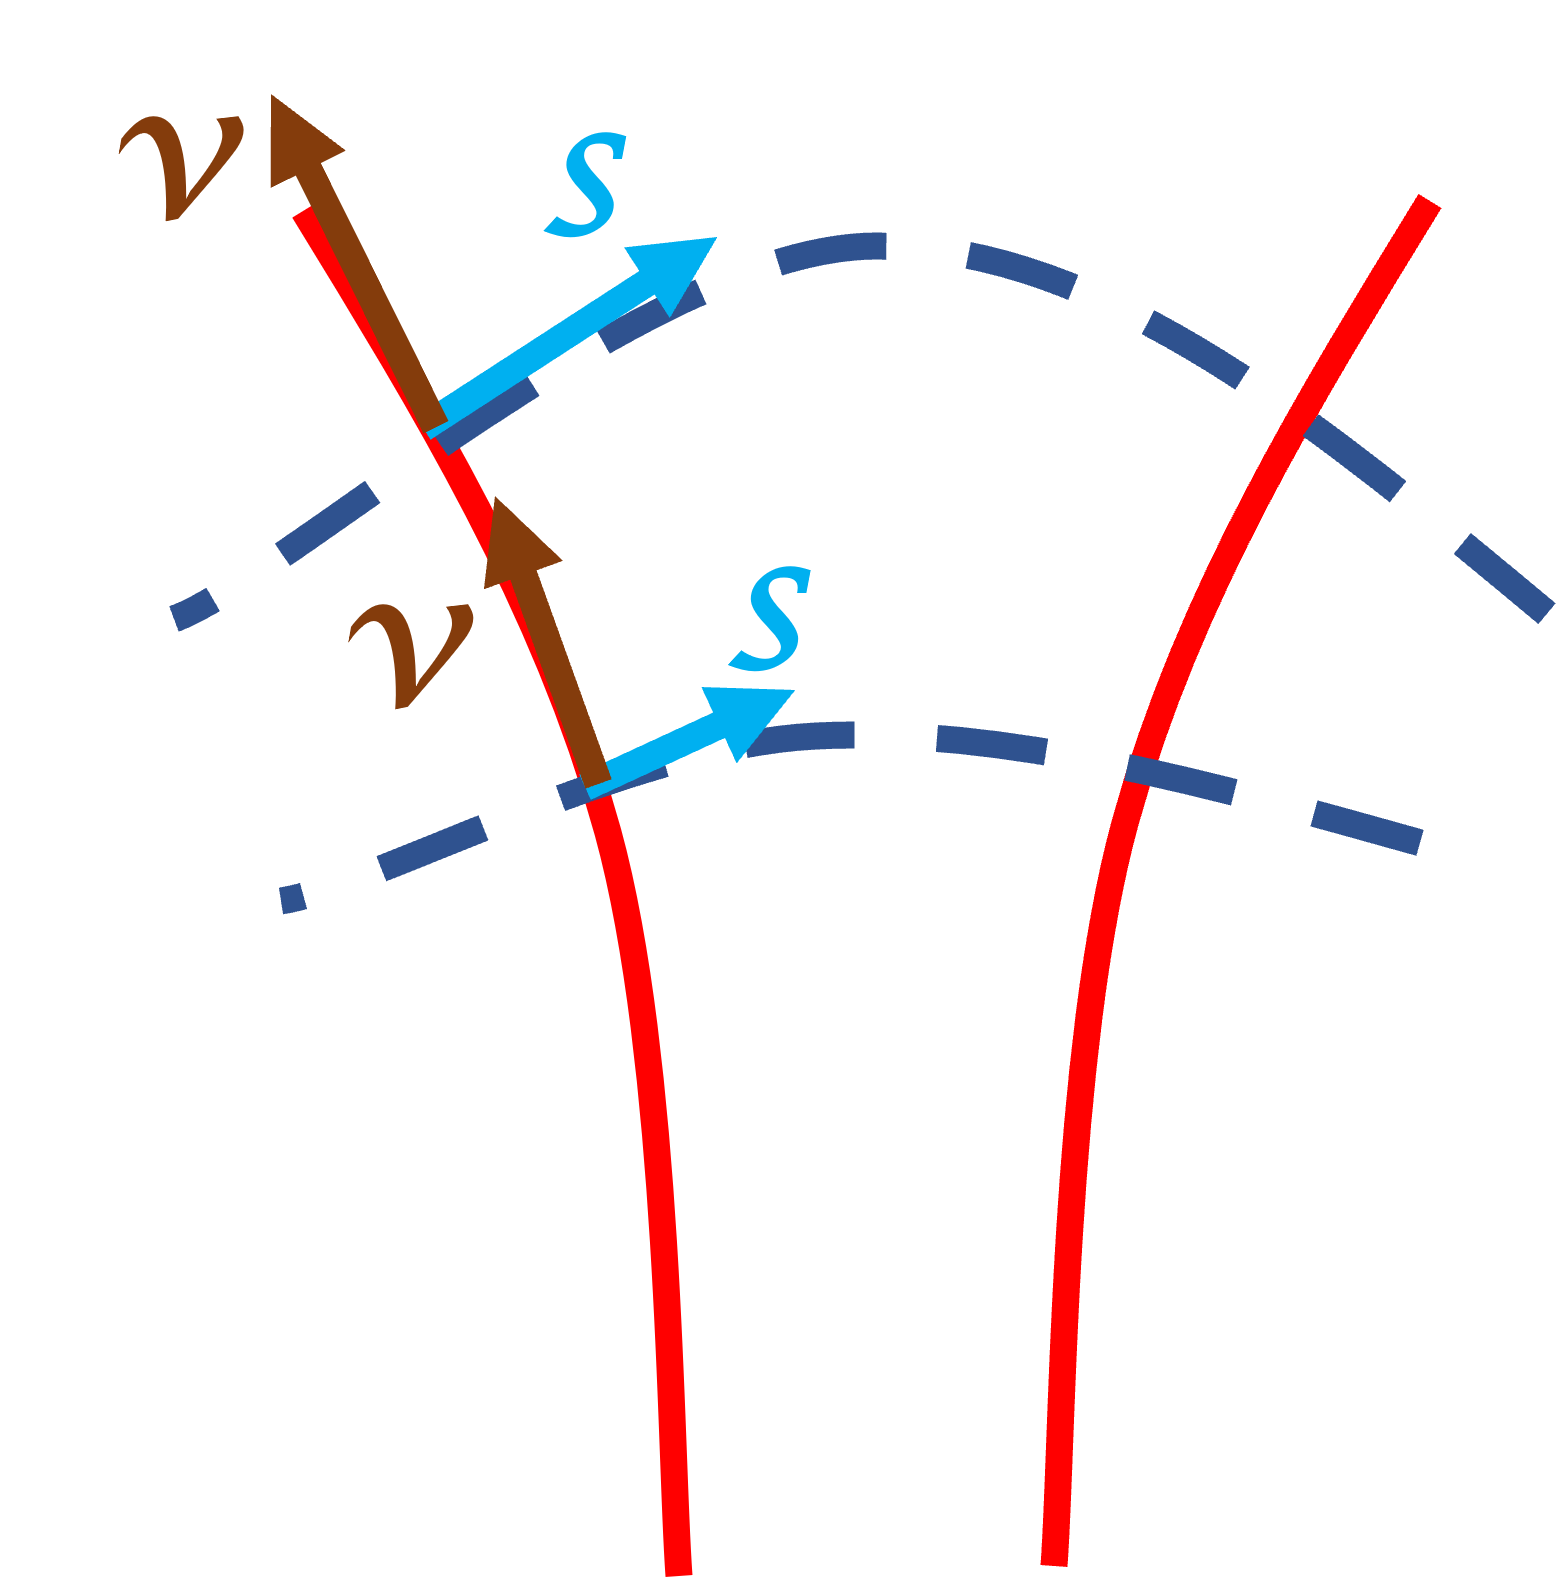
\includegraphics[width=\linewidth]{img04.png}
     \caption{{Case III: We have diverging geodesics (negative curvature)}}
     \label{fig:04}
   \end{minipage}
\end{figure}
\end{frame}

\begin{frame}
\frametitle{Figures Explained}
Note that $\nabla_{\vec{v}}\nabla_{\vec{v}} \vec{s}$ indicates the rate of change of how fast the $\vec{s}$ vector changes with respect to travelling on the geodesic. First we consider the sign. In case I, $\nabla_{\vec{v}}\nabla_{\vec{v}} \vec{s}=0$ (since $\vec{s}$ is uniform throughout the geodesic) . In case II, we have $\vec{s}$ decreasing in magnitude and this decrease decreases continuously. Thus, $\nabla_{\vec{v}}\nabla_{\vec{v}} \vec{s}=0$ is opposite to $\vec{s}$. This yields $\inner{\nabla_{\vec{v}}\nabla_{\vec{v}} \vec{s},\vec{s}<0}$. Using equation \ref{main_eq}, we get $\inner{R(\vec{s},\vec{v}) \vec{v}, \vec{s}}>0$. Likewise, for case III $\inner{R(\vec{s},\vec{v}) \vec{v}, \vec{s}}<0$. This is the intuition behind curvature.
\end{frame}

\begin{frame}
\frametitle{Is This It?}
We have intuitively concluded the form of curvature as $K(\vec{s},\vec{v})=\inner{R(\vec{s},\vec{v}) \vec{v}, \vec{s}}$, which holds true upto a constant. Note that curvature must be independent of the choice of basis. This can be done by suitable normalization.
\pause
Now onwards, we will drop the $\vec{.}$ symbol.\\
Consider a new set of basis $(\tilde{v},\tilde{w})=(av+bw,cv+dw)$ for $a,b,c,d\in\mathbb{R}$. The curvature should not change in this new basis. We will use the fact that 
\begin{align}
\norm{\tilde{v} \wedge \tilde{w}}&=\norm{av+bw \wedge cv+dw}\\
&=\abs{ad-bc}\norm{v \wedge w}
\end{align}
\end{frame}

\begin{frame}
\frametitle{Normalization: Part I}
Now,
\begin{align}
R(\tilde{v},\tilde{w})&=R(av+bw,cv+dw)\\
\label{tensor property 1}
&=R(av,cv)+R(av,dw)+R(bw,cv)+R(bw,dw)\\
\label{tensor property 2}
&=acR(v,v)+adR(v,w)+bcR(w,v)+bdR(w,w)\\
\label{anticommutative property}
&=(ad-bc)R(v,w)
\end{align}
where equations \ref{tensor property 1} and \ref{tensor property 2} use the multi linearity of tensors and equation \ref{anticommutative property} uses the fact that $R(v,w)=-R(w,v)$.
\end{frame}

\begin{frame}
\frametitle{Normalization: Part II}
Using $K(v,w)=\inner{R(v,w) w, v}$ from the previous slides, 
\begin{align}
K(\tilde{v},\tilde{w})&=\inner{R(\tilde{v},\tilde{w}) \tilde{w}, \tilde{v}}\\
\label{riemann property}
&=(ad-bc)\inner{R(v,w) \tilde{w}, \tilde{v}}\\
&=(ad-bc)\inner{R(v,w) av+bw, cv+dw}\\
\label{inner product property}
&=(ad-bc)^2\inner{R(v,w) v, w}
\end{align}
where equation \ref{riemann property} follows from equation \ref{anticommutative property} and equation \ref{inner product property} follows from the axioms of inner product of vectors.\\
\pause
Equation \ref{inner product property} shows that we need to scale down the curvature by $(ad-bc)^2$ in order to normalize it. 
\end{frame}

\begin{frame}
\frametitle{Final Result}
Thus, we can define curvature as
\begin{align}
\label{final result}
K(v,w)&=\frac{\inner{R(v,w) w, v}}{\norm{v\wedge w}^2}
\end{align}
We can show that the above quantity is indeed a tensor and invariant under a change of basis.
\end{frame}